%!TEX root = ../masters_thesis.tex

\section{Application} % (fold)
\label{sec:application}

HistoGlobe is a Web-based Historical Geographic Information System. The Data model and the conceptual model of the user interface were introduced in the first sections of this chapter. This section introduces the underlying database model, a specific implementation of the data model, and the computational model that translates between the conceptual model and the database model. The first part provides an overview about the architecture of the system in section \ref{sub:system_architecture}.
% ... bla bla bla, the rest comes last
% problems
% - support uncertainty

% ------------------------------------------------------------------------------
\subsection{System Architecture} % (fold)
\label{sub:system_architecture}

HistoGlobe uses a classical client-server architecture of a Web-based information system. The user opens the application and interacts with it through the user interface in a Web browser, the \emph{client} side of the system. The Web \emph{server} is a remote computer that hosts the database and the middleware. The user interacts with the interface and the client-side application sends a request to the Web server for new data. The middleware checks the request and queries the necessary data from the database. It transforms the data and sends it back to the client. The interface shows the new information.

\begin{figure}[H]
  \vspace{1em}
  \centering
  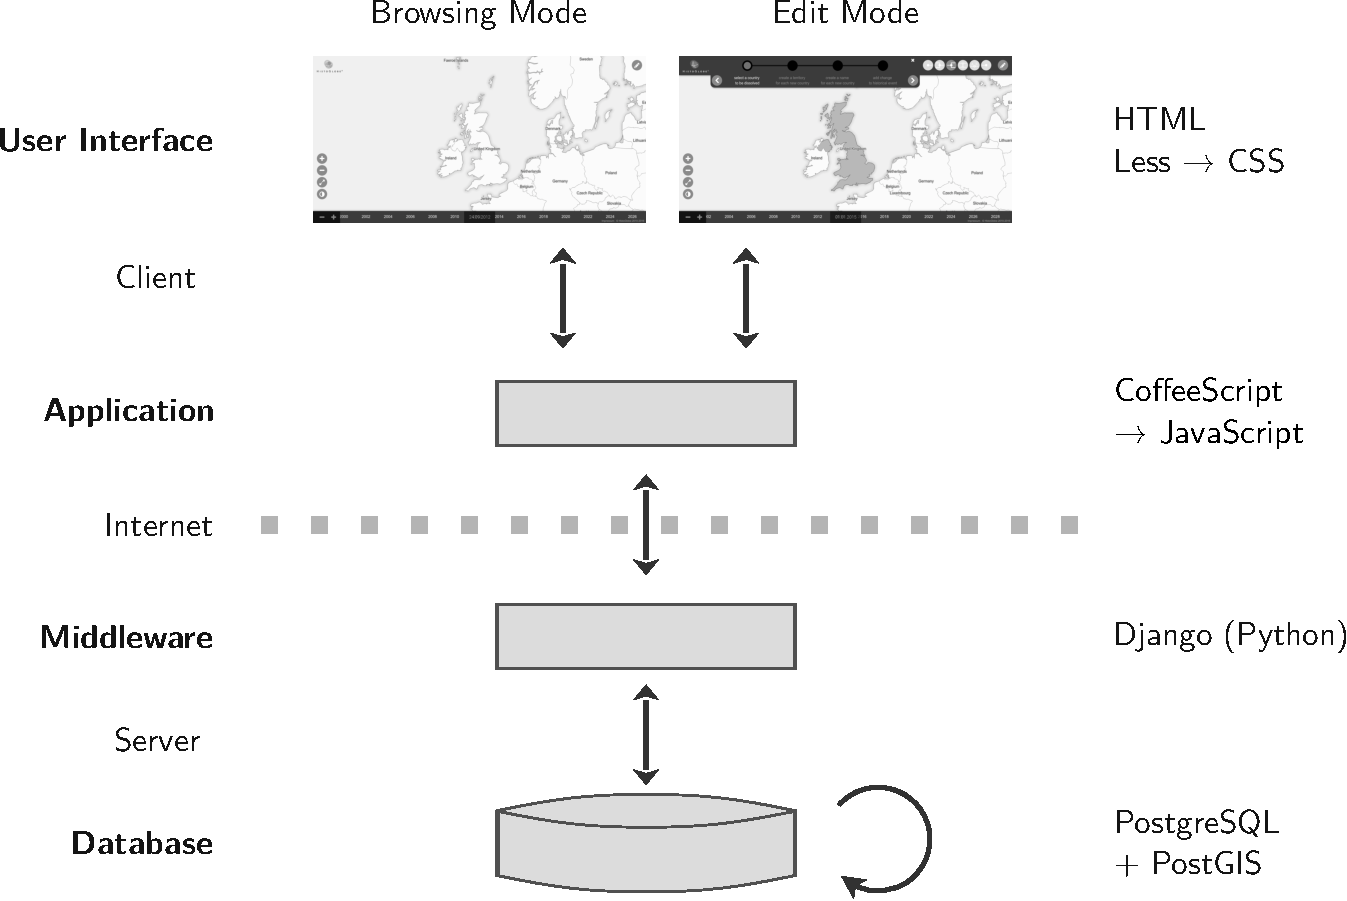
\includegraphics[width=0.7\textwidth]{graphics/development/application/system_architecture}
  \caption{The system architecture of HistoGlobe}
  \label{fig:system_architecture}
\end{figure}

This clear separation between the data, the application and the user interaction in this chapter and in the system follows directly from the \emph{model-view-controller} pattern: One part can be changed independently from the others parts: if the 2D map is replaced by a 3D globe, only the view changes, but the middleware and the database can stay untouched. Likewise, the implementation of a new database technology has no consequences to the view.

% subsection system_architecture (end)

% ------------------------------------------------------------------------------
\subsection{Server-Side Application} % (fold)
\label{sub:server_side_application}

The underlying Hivent Model is implemented on the server-side part of the application. HistoGlobe uses \emph{Django}, a free and open-source web framework
\footnote{
  \emph{Django},
  The Web framework for perfectionists with deadlines,
  URL: \url{https://www.djangoproject.com/},
  last access: 27.05.2016
},
combined with \emph{PostgreSQL}
\footnote{
  \emph{PostgreSQL:},
  The world's most advanced open source database,
  URL: \url{http://www.postgresql.org/},
  last access: 31.10.2015
}
, one of the most popular Object-Relational Database Management Systems introduced in section \ref{sub:object_relational_database_management_systems}, on the server-side of the system. This allows HistoGlobe to take advantage of object-oriented concepts in a stable and fast relational database. Since the database is using a lot of geospatial data, \emph{PostGIS} is used as a spatial database extension for PostgreSQL
\footnote{
  \emph{PostGIS},
  Spatial and Geographic Objects for PostgreSQL,
  URL: \url{http://postgis.net/},
  last access: 27.05.2016
}.

With these tools at hand, the Hivent Model form section \ref{sec:hivent_model}  was implemented in a database model shown in figure \ref{fig:database_model_er}. It is the final result of a highly iterative process that underwent many improvements and adpations to new requirements introduced in the Human Centered Design process. The model is structured in two parts covereing four different domains of the spatio-temporal model: The lower part describes the semantic, spatial and thematic domain of Areas and the upper part represents the temporal domain of Hivents that introduces changes to the Areas.

\begin{figure}[ht]
  \centering
  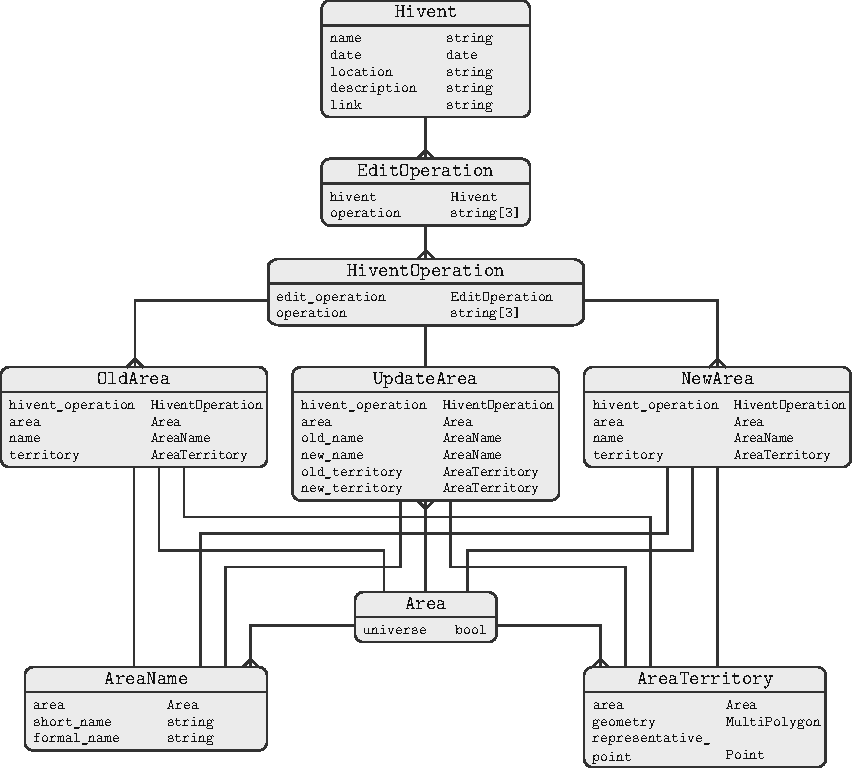
\includegraphics[width=0.8\textwidth]{graphics/development/application/database_model}
  \caption{The Hivent Database Model}
  \small{Each entity additionally has an \texttt{id} attribute, which is omitted for simplification purposes.}
  \label{fig:database_model_er}
\end{figure}

% - - - - - - - - - - - - - - - - - - - - - - - - - - - - - - - - - - - - - - -
\paragraph{Semantic, Spatial and Thematic Domain} % (fold)
\label{par:semantic_spatial_and_thematic_domain}

In the Hivent Model, the entity visible on the map is an Area with a name and a territory, as introduced in section \ref{sec:hivent_model}. In the database model, they are represented by three entities:

\begin{enumerate}
  \item \texttt{Area}: semantic domain defining one identical Area with potentially changing name and territory. The \texttt{universe} attribute is true for $\Omega$, for the other Areas it is false.
  \item \texttt{AreaTerritory}: spatial domain. A polypolygon describes the \texttt{geometry} of the territory and a \texttt{representative\_point} the position of the name label on the map.
  \item \texttt{AreaName}: thematic domain. It is defined by a \texttt{short\_name} and a \texttt{formal\_name}.
\end{enumerate}

% paragraph semantic_spatial_and_thematic_domain (end)

% - - - - - - - - - - - - - - - - - - - - - - - - - - - - - - - - - - - - - - -
\paragraph{Temporal Domain} % (fold)
\label{par:temporal_domain}

The main idea of the model is that the Areas can change over time. These changes are introduced by \texttt{Hivents}, the main entitity of the eponymic model with five attributes: The \texttt{name} and a textual \texttt{description} of the Hivent, the point in time the Hvent happend (\texttt{date}), the Hivent \texttt{location} as a simple string and a \texttt{link} (URL) to the related article, serving as a historical source. Each Hivent can introduce a set of \texttt{EditOperation}s introduced and understood by the user. They consist themselves of a set of low-level \texttt{HiventOperation}s). They replace a set of \texttt{OldArea}s with a set of \texttt{NewArea}s and might update the name or the territory of one specific \texttt{UpdateArea}.

% paragraph temporal_domain (end)

% - - - - - - - - - - - - - - - - - - - - - - - - - - - - - - - - - - - - - - -
\paragraph{Example} % (fold)
\label{par:example}

Figure \ref{fig:database_example_reunification} shows the Hivent Database Model at the example of the German Reunification on 3. October 1990. Before 1990, there were the Areas \texttt{GDR} (``German Democratic Republic'', East Germany) and \texttt{FRG} (``Federal Republic of Germany'', West Germany). A user introduced a Merge operation (\texttt{MRG}) in the Edit Mode between \texttt{FRG} and \texttt{GDR}. The new Area received the short name ``Germany'' and the same formal name ``Federal Republic of Germany'' as previous West Germany. Internally, the Edit Mode translates this to an \texttt{INC} of \texttt{GBDR} into \texttt{FRG} and a subsequent \texttt{NCH} of the \texttt{FRG}. One Area ceases, one Area is updated twice and no new Area is created.

\begin{figure}[ht]
  \vspace{1em}
  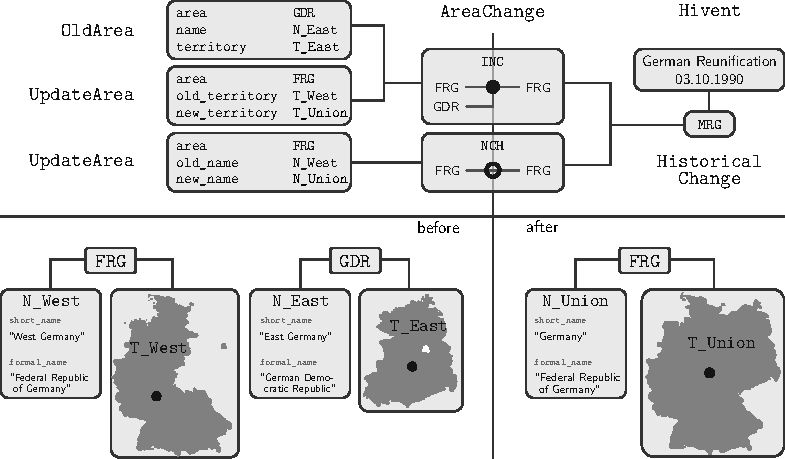
\includegraphics[width=0.9\textwidth]{graphics/development/application/example_reunification}
  \caption{Visualization of the German Reunification in the Hivent Database Model}
  \label{fig:database_example_reunification}
\end{figure}


% paragraph example (end)

% - - - - - - - - - - - - - - - - - - - - - - - - - - - - - - - - - - - - - - -
\paragraph{Initial Dataset} % (fold)
\label{par:initial_dataset}

Section \ref{sub:data_sources} explained the lack of data about historical countries. It is out of the scope of this thesis to create a large testing dataset with the historical countries in the world. The inital dataset consists of the following countries, their names and borders: the 193 UN members and 2 observer states (created by \texttt{CRE} operation) and seven countries with limited international recognition: Kosovo, Transnistria, South Ossetia, Abkhazia, Nagorno-Karabakh, Somaliland and Sahrawi Arab Democratic Republic, see section \ref{par:un_non_members_with_limited_recognition}) (created by \texttt{DIS} operations from their homeland on the day of their declaration of independence).

% paragraph initial_dataset (end)

% - - - - - - - - - - - - - - - - - - - - - - - - - - - - - - - - - - - - - - -
\paragraph{Middleware} % (fold)
\label{par:middleware}

The Django web framework provides \emph{view} classes as the middleware that receives requests from the client, processes them, queries the necessary data from the database and returns an \texttt{HttpResponse} back to the client. In the naive implementation of the system, the middleware provides only two views for the two use cases:

\begin{enumerate}
  \item \textbf{\texttt{get\_all}} is initially called by the client side on loading the web service. The server responds to this \texttt{HttpRequest} with all data from the database in one \emph{JSON} object. While this behaviour is not scalable, for the initial dataset it was sufficient: The data was loaded in 3.5 seconds.
  \item \textbf{\texttt{save\_edit\_operation}} is called by the client after an Edit Operation has been completely created in the Edit Mode. In the last step, the client assembles the relevant data: the associated \texttt{Hivent} and \texttt{HiventOperation}s), data about each \texttt{OldArea}, \texttt{UpdateArea} and \texttt{NewArea}. The view checks the data for integrity and stores them in the database. The method returns to the client a confirmation and a set of final \texttt{id}s for the entities stored in the database.
\end{enumerate}

% paragraph middleware (end)

% subsection server_side_application (end)

% ------------------------------------------------------------------------------
\subsection{Client-Side Application} % (fold)
\label{sub:client_side_application}

The main application of HistoGlobe runs on the client. As introduced in section \ref{sec:histoglobe}, the software is built upon a module system. The modules used in this this implementation of HistoGlobe are emphazised in \textbf{bold} in the class diagram in figure \ref{fig:class_diagram}. The classes are structured by their functionality regarding the Model-View-Controller pattern.

\begin{sidewaysfigure}[p]
  \centering
  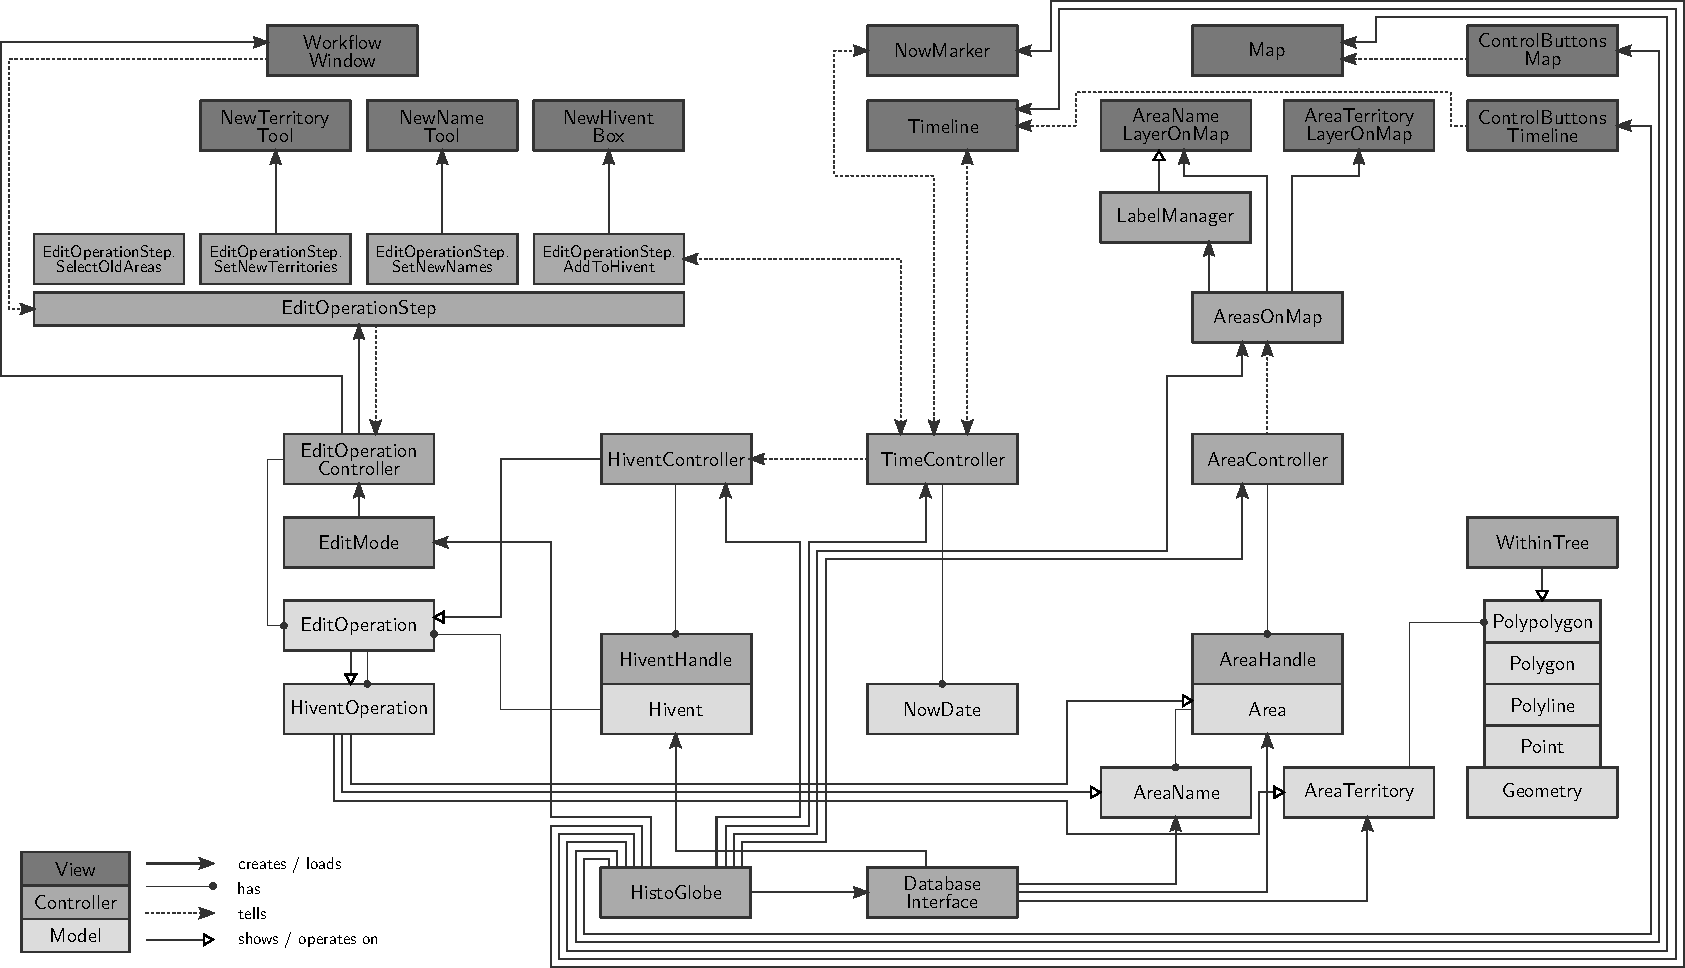
\includegraphics[width=0.95\textwidth]{graphics/development/application/class_diagram}
  \vspace{1em}
  \caption{Class Diagram of HistoGlobe}
  \label{fig:class_diagram}
\end{sidewaysfigure}

\newpage % forces the figure to be on the next page, because [H] does not work
% - - - - - - - - - - - - - - - - - - - - - - - - - - - - - - - - - - - - - - -
\paragraph{Initialization} % (fold)
\label{par:initialization}

The main HistoGlobe instance in the bottom initializes all modules, mainly the interface elements, the controllers and the \texttt{DatabaseInterface}. This class communicates with the middleware (section \ref{par:middleware}), loads data from and stores data in the database. Initially, each \texttt{Hivent} and the related \texttt{EditOperation}s and \texttt{HiventOperation}s are created. Each \texttt{HiventOperation} is assembled by its associated set of \texttt{OldArea}s, \texttt{NewArea}s and the \texttt{UpdateArea} from the datase model in  figure \ref{fig:database_model_er}. Afterwards, each \texttt{Area}, \texttt{AreaName} and \texttt{AreaTerritory} is loaded. A double-link is established to their associated \texttt{HiventOperation}s via the \texttt{startOperation}, \texttt{updateOperation} and \texttt{endOperation}. Therefore, each \texttt{HiventOperation} knows which \texttt{Area}s, names and territories it creates, updates and ceases -- and vice verse each \texttt{Area}, \texttt{AreaName} and \texttt{AreaTerritory} knows which \texttt{HiventOperation} manipulates its development.

% paragraph initialization (end)

% - - - - - - - - - - - - - - - - - - - - - - - - - - - - - - - - - - - - - - -
\paragraph{Executing temporal changes} % (fold)
\label{par:executing_temporal_changes}

HistoGlobe visualizes time on the interactive \texttt{Timeline} and the static \texttt{NowMarker} showing the current date of the application: the \texttt{NowDate}. Both view classes can manipulate the current date by moving the \texttt{Timeline} or entering a date into the \texttt{NowMarker}. The \texttt{TimeController} stores the \texttt{NowDate} and tells all other modules if the current visualization has changed.

\begin{figure}[ht]
  \vspace{1em}
  \centering
  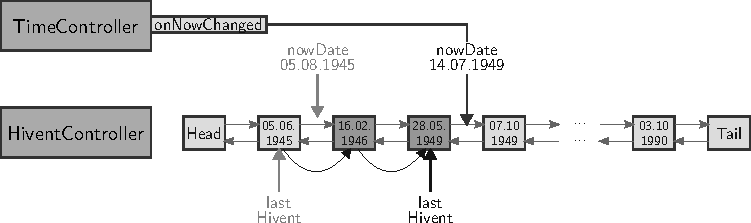
\includegraphics[width=0.8\textwidth]{graphics/development/application/hivent_controller}
  \caption{Detecting the next Hivent that happens in the \texttt{HiventController}}
  \label{fig:hivent_controller}
\end{figure}

The core of the Hivent-based implementation is the \texttt{HiventController}. Figure \ref{fig:hivent_controller} illustrates how it works: The controller stores a reference to each \texttt{Hivent} chronologically in a doubly-linked list, i.e. each \texttt{Hivent} knows the historically next and previous \texttt{Hivent}. Additionally, the controller stores a pointer to the last \texttt{Hivent} in the list that has happened and a copy of the current date. It listens to the \texttt{TimeController} -- if the \texttt{NowDate} changes, the \texttt{HiventController} checks for the next \texttt{Hivent} if it has happened: The controller compares this new date with its current date checks if the \texttt{Hivent.date} is in between these two dates. If this is the case, the \texttt{Hivent} happens and all the \texttt{EditOperations} associated to this \texttt{Hivent} are executed on the map. The \texttt{HiventController} updates the pointer to the \texttt{Hivent} and checks for the next one until the next \texttt{Hivent} is outside this time span. If the \texttt{nowDate} from the \texttt{TimeController} is before the current date of the \texttt{HiventController}, it checks for \texttt{Hivents} backwards through the list and executes all the \texttt{EditOperations} backwards. This simple data structure allows to effectively and efficiently manage temporal changes of \texttt{Area}s on the map. On initialization of the system, after the \texttt{DatabaseInterface} loaded all the data, the \texttt{HiventController} starts this process: All \texttt{Hivent}s in the list from the beginning until the \texttt{NowDate} of the \texttt{TimeController} are happening one after the other.

An \texttt{EditOperation} diverts the execution to all its related \texttt{HiventOperations}. They are the integral objects that change the status on the map. The main part of its source code, the \texttt{execution} function is shown in listing \ref{lst:hivent_operation}. As mentioned above, there are two change directions: forward and backward. If an \texttt{HiventOperation} is to be executed forwards, the following three steps happen:

\begin{enumerate}
  \item For each \texttt{newArea}, the \texttt{AreaName} and the \texttt{AreaTerritory} that the \texttt{Area} has in the moment it gets historically created are associated to the \texttt{Area}. Afterwards, the \texttt{Area} is shown on the map: The \texttt{AreaHandle} associated to the \texttt{Area} has a function that tells the \texttt{AreaNameLayerOnMap} and \texttt{AreaTerritoryLayerOnMap} to be shown.
  \item For each \texttt{oldArea}, the opposite happens: the name and territory are detached from the \texttt{Area} and the \texttt{AreaHandle} hides the \texttt{Area} from the map.
  \item In the \texttt{updateArea} the \texttt{AreaName} or \texttt{AreaTerritory} is replaced by the \texttt{newName} respectively \texttt{newTerritory}. The \texttt{update} method of the \texttt{AreaHandle} updates the respective layers on the map.
\end{enumerate}

In case the operation happens backwards, \texttt{oldAreas} and \texttt{newAreas} are swapped and the \texttt{updateArea} uses the \texttt{oldName} respectively \texttt{oldTerritory} instead.

\begin{center}
\begin{minipage}[t]{0.8\textwidth}
\begin{lstlisting}[language=coffeescript,
  caption=Execution of an \texttt{HiventOperation},
  label=lst:hivent_operation]
class HiventOperation

  constructor: (data) ->
    #...

    @oldAreas   = []  # {area, name, territory}
    @newAreas   = []  # {area, name, territory}
    @updateArea = {}  # {area, oldName, newName, oldTerritory, newTerritory}

    #...

  execute: (direction) ->

    if direction is 1

      for newArea in @newAreas
        newArea.area.name =       newArea.name
        newArea.area.territory =  newArea.territory
        newArea.area.handle.show()

      for oldArea in @oldAreas
        oldArea.area.name =       null
        oldArea.area.territory =  null
        oldArea.handle.hide()

      if @updateArea
        if @updateArea.newName
          @updateArea.area.name =      @updateArea.newName
        if @updateArea.newTerritory
          @updateArea.area.territory = @updateArea.newTerritory
        @updateArea.area.handle.update()

    else # direction is -1 => backward change
      # same as above, just each 'new' is replaced by 'old' and vice versa
\end{lstlisting}
\end{minipage}
\end{center}

% paragraph executing_temporal_changes (end)

% - - - - - - - - - - - - - - - - - - - - - - - - - - - - - - - - - - - - - - -
\paragraph{EditMode} % (fold)
\label{par:editmode}

The Edit Mode is the main contribution of this thesis to the HistoGlobe project. Its interface was introduced in section \ref{sub:web_based_prototype}, this section shortly explains its implementation: When the user clicks a button of an Edit Operation in the upper right corner of the Edit Mode interface, internally a \texttt{EditOperationCreator} sets up the \texttt{WorkflowWindow} in the interface and the first \texttt{EditOperationStep} for this operation. Each of the four steps have different tasks. They area introduced in section \ref{sub:edit_workflow}. The \texttt{EditOperationCreator} stores the data for each step (selected Areas, newly defined territories and names) in an object. Each step can access this object and manipulate its content. It was especially difficult to design each action to be fully reversible. For that purpose, an associated inverse of the action was stored in an \texttt{UndoManager} that works like a stack. If the user clicks the back button in the Workflow Window, the last action of the stack gets executed. When the last stage of the workflow (\texttt{AddToHivent}) is completed, the \texttt{EditOperationCreator} assembles the \texttt{HiventOperations} from the data gathered in the task. It sends it along with the associated \texttt{Hivent} to the server and finishes the operation.

% paragraph editmode (end)

% - - - - - - - - - - - - - - - - - - - - - - - - - - - - - - - - - - - - - - -
\paragraph{Within-Tree} % (fold)
\label{par:within_tree}

One particular problem of the territory of an Area is that the associated polypolygon can have holes to account for enclaves and exclaves. They can even be nested (second-order enclaves, third-order enclaves, etc.), as in the example of Baarle-Nassau and Baarle-Hertog at the border between the Netherlands and Belgium
\footnote{
  \emph{The Curious Case of Baarle-Nassau and Baarle-Hertog},
  kaushik, 06.11.2012,
  \url{http://www.amusingplanet.com/2012/11/the-curious-case-of-baarle-nassau-and.html},
  last access: 31.05.2016
}.
The \texttt{NewTerritoryTool} has to ensure that the drawn polygons are not self-intersecting and that no two polygons for one territory partially overlap each other. If they fully overlap, then they are holes in the polygon. A polygon consist of one \emph{outer ring}, a closed polyline forming the boundary of the polygon, and a set of \emph{inner rings}, closed polylines defining the holes in the polygon. Second-order enclaves are new polygons that happen to be positioned inside the inner rings of the other polygon. They can themselves have inner rings, which represent third-order enclaves, etc.

In order to supported nested holes, the \emph{WithinTree} is introduced. The idea of the tree is to set up an hierarchical structure of polygons that contain each other. An example Within-Tree for a random set of polygons can be seen in figure \ref{fig:within_tree}.

\begin{figure}[ht]
  \vspace{1em}
  \centering
  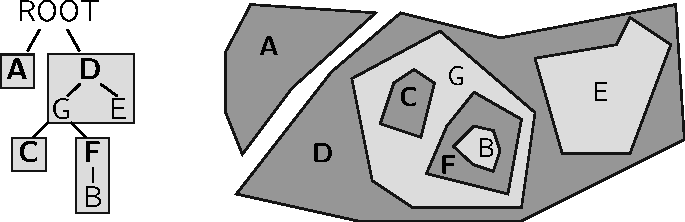
\includegraphics[width=0.6\textwidth]{graphics/development/application/within_tree}
  \caption{The Within-Tree (left) for the set of polygons (right)}
  \label{fig:within_tree}
\end{figure}

The algorithm for inserting a polygon as a node into the tree is shown in listing \ref{lst:within_tree_insertion}. After the tree has been set up, the correct structure of polygons can be obtained by traversing the tree in the following custom order:

\begin{compactenum}
  \item Remove the first child $F$ of the root node and all its children $C$ from the tree.
  \item Insert each child of each $C$ as a direct child of the root node.
  \item Create a new polygon with $F$ as the outer ring and each $C$ as an inner ring.
  \item Repeat until the tree is empty.
\end{compactenum}



\begin{center}
\begin{minipage}[t]{0.8\textwidth}
\begin{lstlisting}[language=coffeescript,
  caption=Insertion of a polygon node into the Within-Tree,
  label=lst:within_tree_insertion]
insert: (newNode, parentNode) ->

  ## PREPARATION
  # case 1) newNode also in 1 child of parentNode  -> withinChild
  # case 2) 1+ children of parentNode in newNode   -> containChildren
  # case 3) no hierarchical relation between newNode and any other node

  withinChild =     null
  containChildren = []

  for childNode in parentNode.children

    if newNode.isWithin childNode                   # check if case 1)
      withinChild = childNode
      break # no other hierarchical relation to any other child possible

    else if childNode.isWithin newNode              # check if case 2)
      containChildren.push childNode

  ## EXECUTION

  if withinChild                                    # case 1)
    @insert newNode, childNode

  else                                              # cases 2 and 3)
    # newNode is not in any child of parentNode => place it underneath
    @_nodes.push newNode
    newNode.setParent parentNode
    parentNode.addChild newNode

    for containChild in containChildren             # case 2)
      # => detach from parent node and place them as children of newNode
      containChild.setParent newNode
      newNode.addChild containChild
      parentNode.removeChild containChild
\end{lstlisting}
\end{minipage}
\end{center}

% paragraph within_tree (end)

% - - - - - - - - - - - - - - - - - - - - - - - - - - - - - - - - - - - - - - -
\paragraph{LabelManager} % (fold)
\label{par:labelmanager}

A major visualization problem that was sufficiently solved is the thesis is the label collision problem: Each active Area has both a territory and a name that should be shown on the map. Since no territories can overlap (precondition \ref{axm:unique_coverage}), they can all be shown. This is not true for the names of the Areas: The \texttt{short\_name} of the \texttt{AreaName} is placed as a label in the \texttt{representative\_point} of the \texttt{AreaTerritory}. Labels can overlap, because they can extend beyond their territory. To avoid this, some labels have to be hidden. A \texttt{LabelManager} decides for each label if it is shown or hidden. Each label gets an additional set of attributes:

\begin{compactitem}
  \item \texttt{isVisible}: status variable if the label is shown or not
  \item \texttt{priority}: the ``importance'' of the label determined by the size of the territory
  \item \texttt{boundingBox}: width and height of the text plus 5 pixel padding
  \item \texttt{coveredBy}: a list of higher-priority labels that cover this label
  \item \texttt{covers}: a list of lower-priority labels that are covered by this label
\end{compactitem}

Label $A$ covers label $B$ if their bounding boxes intersect and $A$ has a higher priority. The labels are stored in a doubly-linked \texttt{labelList} in a descending order by priority. The algorithm is based on the following heuristic: \emph{A label is shown unless it is covered by an higher-priority label}.

When a new label is supposed to be shown on the map, it is inserted into the \texttt{LabelManager} like this: The correct position of the label in the \texttt{labelList} is found by checking with each element in descending priority if they overlap and if the priority is still higher. As soon as the first label with a lower priority is found, the new label is inserted before this label in the list. If there was a higher-priority label before that covered it, the new label is hidden -- else it is shown. In the latter case all lower-priority labels are checked if they are covered by the new label -- if so, they are hidden.

If an Area ceases also its name is hidden from the map. Additionally, the old label is removed from the \texttt{labelList}. Each label that was previously covered by the old label is not not covered by it anymore. If no other label is still covering it, the label can be shown now.

If the user zooms the map, the \texttt{LabelManager} has to update the visibility status of each label. Zooming in  means that each label has more space to its neighbors. No label has to be hidden, but a hidden labels can be shown if it is not covered by any other label anymore. Vice versa, if the user zooms out, the labels have less space to their neighbors. No label can be shown now, but a visible labels needs to be hidden if is covered by at least one other label now.

\begin{figure}[ht]
  \centering
  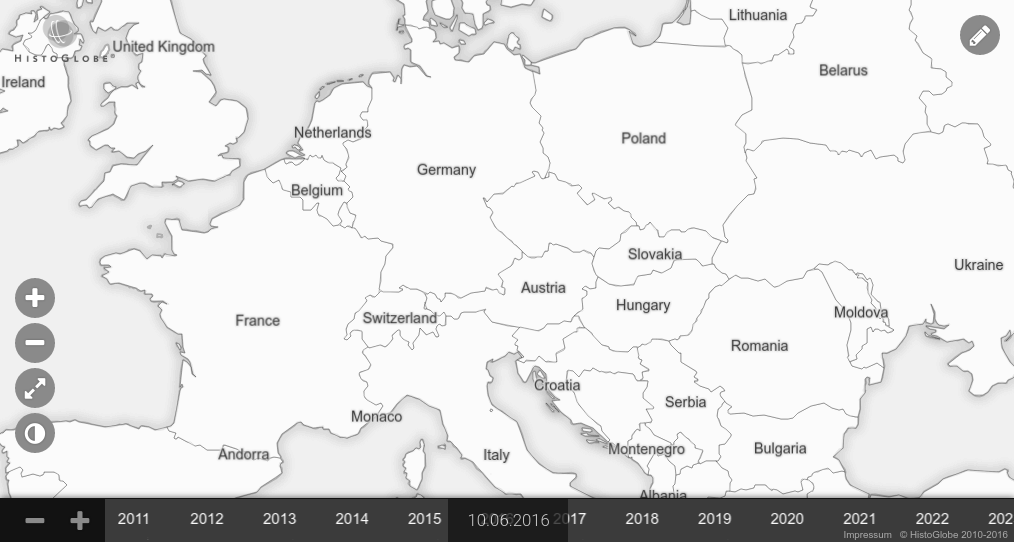
\includegraphics[width=0.7\textwidth]{graphics/development/application/label_manager.png}
  \caption{The resulting labels on the map in Europe 2016}
  \label{fig:label_manager}
\end{figure}

Figure \ref{fig:label_manager} shows the result of the \texttt{LabelManager} on the map of Europe in 2016. It is obvious that no two labels collide which was the main motivation for the algorithm. Also, the labels of the large countries Ukraine, Poland, Germany, France and the United Kingdom are shown. However, the label ``Czech Republic'' is hidden, because its bounding box intersects with the label ``Germany''. On the other hand the labels of Monaco and Andorra are shown, although they are rather insignificant. But since there is enough space around them, they are shown. The \texttt{LabelManager} sufficiently serves the purpose of this thesis.

% paragraph labelmanager (end)

% subsection client_side_application (end)

% section application (end)